\documentclass[conference]{IEEEtran}
\IEEEoverridecommandlockouts
% The preceding line is only needed to identify funding in the first footnote. If that is unneeded, please comment it out.
\usepackage{cite}
\usepackage{amsmath,amssymb,amsfonts}
\usepackage{algorithmic}
\usepackage{graphicx}
\usepackage{textcomp}
\usepackage{xcolor}
\usepackage{hyperref}
\usepackage{float}
\usepackage[table]{xcolor}

\def\BibTeX{{\rm B\kern-.05em{\sc i\kern-.025em b}\kern-.08em
    T\kern-.1667em\lower.7ex\hbox{E}\kern-.125emX}}
\begin{document}

\title{Heart Disease Prediction \\with \\different machine learning models}

\author{\IEEEauthorblockN{Paweł Narwojsz}
\IEEEauthorblockA{197977}
\and
\IEEEauthorblockN{Jakub Bot}
\IEEEauthorblockA{197839}
\and
\IEEEauthorblockN{Piotr Kaczorowski}
\IEEEauthorblockA{197736}
\and
\IEEEauthorblockN{Paweł Rietz}
\IEEEauthorblockA{197879}
}

\maketitle

% \begin{abstract}
% This study evaluates the effectiveness of several machine learning classifiers in predicting heart disease. 
% Models are trained and validated on a public dataset using cross-validation. 
% Performance is assessed using standard metrics. 
% The results provide insight into the most reliable methods for early heart disease prediction.
% \end{abstract}



% \begin{IEEEkeywords}

% % to delete?
% %component, formatting, style, styling, insert
% \end{IEEEkeywords}

\section{Introduction}

Cardiovascular diseases (CVDs) are among the leading causes of death worldwide, prompting a growing interest in 
early diagnosis and prevention using data-driven approaches. With the increasing availability of medical datasets, 
machine learning (ML) has become a powerful tool for predicting the likelihood of heart disease based 
on clinical parameters such as age, cholesterol level, blood pressure and other risk factors.

The goal of this project is to evaluate and compare the performance of various classification models 
in predicting the presence of heart disease. In particular, we explore popular supervised learning 
algorithms including Random Forest (RF), Support Vector Machine (SVM), AdaBoost (ADA) and Naive Bayes. Each model 
is trained and validated on a publicly available heart disease dataset using cross-validation and a 
range of evaluation metrics such as accuracy, precision, recall, and the Area Under the ROC Curve (AUC).
\\ \\
In our problem, the classification task is to predict whether a patient has heart disease or is healthy.
Incorrect predictions in this context can lead to serious consequences. Therefore, we emphasize \textbf{minimizing 
false negatives} (i.e., failing to identify a patient with heart disease), which are more critical in a 
medical setting than false positives (i.e., incorrectly diagnosing a healthy patient). 
We are thus willing to accept a slightly lower overall accuracy if the model rarely misclassifies 
diseased patients as healthy.


\section{Methodology}
Data used for the analyse of used algorithms has been 
%! I'm not sure - check this
obtained from the UCI Machine Learning Repository \footnote{\url{https://archive.ics.uci.edu/ml/datasets/heart+Disease}}.
The dataset contains various clinical features such as age, sex, chest pain type,
resting blood pressure, cholesterol, fasting blood sugar,
resting electrocardiographic results, maximum heart rate achieved,
exercise induced angina, ST depression, and others. Prior to training
data was divided between train set and test set. First one has been used
for model training the other one to test accuracy of used algorithm.

\section{Evaluation Metrics and Models Description}
\subsection{Models Description}
We compared the performance of the following classification models:
\begin{itemize}
    \item \textbf{Random Forest (RF)}: An ensemble learning method that constructs multiple decision trees during training and aggregates their outputs through majority voting. It is robust to overfitting and can handle large datasets with high dimensionality.
    \item \textbf{Support Vector Machine (SVM)}: Classifier that finds the optimal hyperplane to separate different classes in the feature space.
    \item \textbf{AdaBoost (ADA)}: An ensemble method that combines multiple weak classifiers, typically decision stumps, into a strong one by focusing more on previously misclassified instances.
    \item \textbf{Naive Bayes}: A probabilistic classifier based on Bayes' theorem, assuming independence among features. It is simple, fast, and effective for large datasets, but may struggle with correlated features.
    \item \textbf{Random Forest and ADA with Class Weights}: Models that incorporates class weighting, allowing the model to pay more attention to misclassified instances from the minority class. This typically leads to improved recall or precision.
\end{itemize}
\subsection{Evaluation Metrics}
To evaluate the performance of the models, we used the following standard metrics:
\begin{itemize}
    \item \textbf{Accuracy}: The proportion of correct predictions made by the model to total number of samples.
    \item \textbf{AUC (Area Under the ROC Curve)}:  Represents the model’s ability to distinguish between classes. A higher AUC indicates better discriminative performance.
    \item \textbf{Recall}: The proportion of correctly predicted positive cases out of all actual positives. 
    In the context of heart disease prediction, this is especially important, 
    as a low recall means many true cases are missed (false negatives).
\end{itemize}


\section{Implementation}

The implementation is developed using the python language. The model training
is done using the scikit-learn library, a modern and high performance library, containing
most of the learning algorithms used in this study.

The initial data gets split into testing and training datasets, with training
dataset taking 75\% of the whole dataset. The test dataset containing 25\% respectively.

All of the datasets are split between parameters, and the outcome
(In our case, if the patient with given parameters has died).

Regression models were trained with parameters given below

\textbf{Random Forest:}
\begin{itemize}
    \item Number of trees: 100
    \item Maximum forest depth: 5
\end{itemize}

\textbf{Support Vector Machine:}
\begin{itemize}
    \item Regularization parameter (C): 1
\end{itemize}

\textbf{AdaBoost:}
\begin{itemize}
    \item Number of estimators: 50
    \item Learning rate: 0.5
\end{itemize}

\textbf{Naive Bayes:}
\begin{itemize}
    \item Variance smoothing: $10^{-9}$
\end{itemize}

\textbf{Random Forest (With Class Weights):}
\begin{itemize}
    \item Number of trees: 100
    \item Maximum forest depth: 5
    \item Class weights: \{Healthy: 1, Diseased: 10\}
\end{itemize}

\textbf{AdaBoost (With Class Weights):}
\begin{itemize}
    \item Number of estimators: 50
    \item Learnign rate: 0.5
    \item Class weights: \{Healthy: 1, Diseased: 5\}
\end{itemize}

Parameters were tuned to yield the best results %! very subjective xddd

The last two models are supplemented with class weights, whose role is to minimize false-positives of Classes with higher weight.

Additional libraries that were used:
\begin{itemize}
    \item Pandas, for numerical operations
    \item Seaborn, to display the data
    \item Matplotlib, to draw the plots
\end{itemize}

\section{Regression Results}

The results of all models have been evaluated using 10-fold cross-validation to ensure greater reliability.
The accuracy of each model has been calculated and is presented in Figure \ref{fig:accuracy}. 


Below is the figure with data of each model accuracy:
\begin{figure}[H]%[htbp]
    \centering
    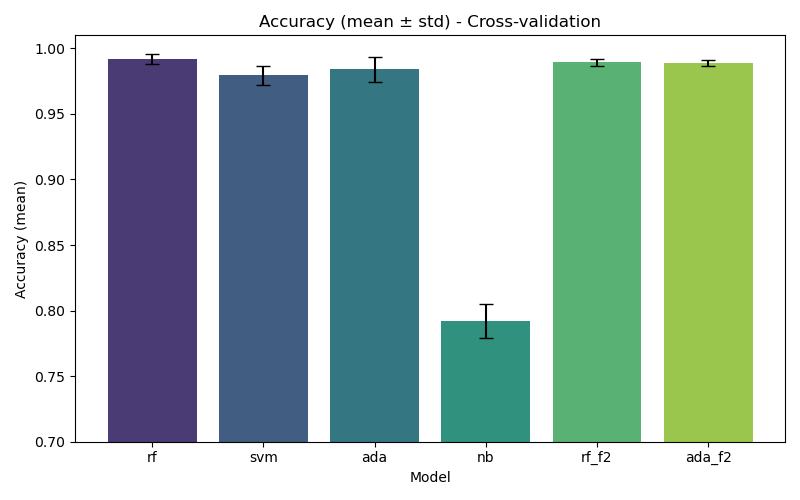
\includegraphics[width=0.5\textwidth]{../src/plots/accuracy_cv_plot.png}
    \caption{Accuracy comparison of different classification models used in heart disease prediction.}
    \label{fig:accuracy}
\end{figure}

As we can observe, the accuracy of models: [rf, svm, rf\_2, ada\_2] averages around 97-99\% accuracy.
The Naive Bayes method yields the worst results by far, scoring +-80\%, significantly worse than other
mentioned methods.
\\ 

To provide a more comprehensive comparison, the results in Table~\ref{auc_tab} include not only the average values of key metrics,  
but also their standard deviations, calculated across all cross-validation folds. \\
The lower the SD, the more stable and reliable behavior of the model is.


\begin{table}[H]
    \caption{Evaluation metrics (mean $\pm$ standard deviation)}
    \label{auc_tab}
    \begin{center}
        \begin{tabular}{|c|c|c|c|}
            \hline
            \textbf{Model} & \textbf{Accuracy} & \textbf{AUC} & \textbf{Recall}  \\
            \hline
            Random Forest & 99.2\% ± 0.4 & 99.9\% ± 0.1 & \textcolor{green}{97.8\% ± 1.3}  \\
            SVM & 97.9\% ± 0.7 & 99.0\% ± 0.5 & 96.5\% ± 1.0 \\
            AdaBoost & 96.0\% ± 1.0 & 98.9\% ± 0.4 & \textcolor{blue}{92.2\% ± 2.8}  \\
            Naive Bayes & 79.2\% ± 1.3 & 88.0\% ± 1.3 & 49.6\% ± 3.1 \\
            Random Forest (Weights) & 98.9\% ± 0.3 & 99.9\% ± 0.1 & \textcolor{green}{98.0\% ± 0.8} \\
            AdaBoost (Weights) & 98.6\% ± 0.3 & 99.3\% ± 0.4 & \textcolor{blue}{97.8\% ± 0.7} \\
            \hline
        \end{tabular}
    \end{center}
\end{table}
Table \ref{auc_tab} summarizes the accuracy, AUC and recall metrics
for each tested model, highlighting their performance in
classifying the data accurately. The Random Forest model achieved
the highest percentage of desired outputs on the test data.
Another model with excellent performance is AdaBoost,
which attained an AUC score above 99\%. 
Looking at the results of models with class weights, 
we can see that they achieve higher recall scores compared to their non-weighted counterparts, with lower standard deviation.
In the case of AdaBoost, the improvement was particularly significant,
because overall accuracy also improved, showing the positive effect of incorporating class weights.
\\
\newpage
The figure below shows confusion matrices for ADA model compared with and without class weights. It illustrates
how significant might be the difference in results when using class weights.
\begin{figure}[H]
    \centering
    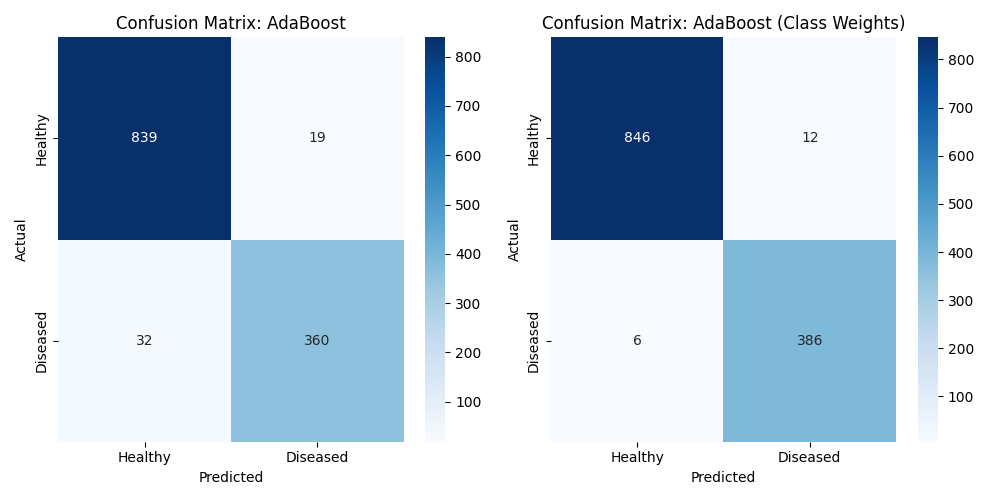
\includegraphics[width=0.5\textwidth]{../src/plots/conf_matrices_adaboost_comparison.png}
    \caption{Confusion matrices for AdaBoost model, with and without class weights.}
    \label{fig:confusion_matrices}
\end{figure}
As shown above, incorporating class weights reduces the number of false negatives, which is critical
for identifying diseased patients. This confirms the earlier observation that using class weights improves recall
without significantly sacrificing overall accuracy. For the RF models the differences are not as pronounced(because
it originally has high recall), but still noticeable.

\section{Best Models}
Based on the most important evaluation metrics of analysed models, both the \textbf{Random Forest}
and \textbf{AdaBoost} models with \textbf{class weights} 
stand out as the best performers for the task of heart disease prediction. 
Other models, such as SVM or standard versions of
RF and ADA does also perform well and achieve high accuracy. However, they perform worse in terms of the recall 
- a crucial metric in medical applications -
and also exhibit higher standard deviation, indicating less stability across different data splits.

\section{Conclusion}

The simulation shows promising results. With +- 99\% overall accuracy for best models, and $<$2\% false negatives rate,
the AI models may serve as a great tool for medical professionals to help correcty identify heart diseases. \\

Two learning approaches standed out boasting high accuracy and low false negative rates, the ones being Random Forest and AdaBoost.
Introducing weights into the learning process, effectively reduced false negative flags, which is crucial for medical use. This
modification didn't degrade the overall accuracy of the models as well. \\

The data used to train the models, included comprehensive measurements such as creatinine phosphokinase levels
in blood, which may not be readily available when diagnosing a patient, which makes the model less usable, when
little or no data are given about the patient. \\

Another issue which might arise is the invisible nature of the model's thinking process.
When getting a result, little is known about how the decision was made, and with what degree
of confidence. In such a critical sector, it creates great uncertainity about model's decisions \\

In conclusion, the machine learning approach shows great potential of correctly identifying heart diseases.
The models show high overall accuracy, and little false negatives. On the other hand, the data used was very comprehensive,
and little is known about the performance of the models with less training data. Models with greater decision making visability
would be more desired, giving medical professionals crucial information needed to make the final decision.

\end{document}